% !TeX spellcheck = en_GB
\section{Finding Crossings}
Percolations are complicated objects.
Even for finite percolations, say one with side $n$, depth $d$ in $D$ dimensions, here are $2^{\left( n^D \right)^d}$ possibilities.
This grows extremely rapidly, and makes theoretical results hard to derive.

Therefore, we choose to study these object further with numerical simulations.

\paragraph{Examples}
To see how complicated finding crossing on percolation becomes when $d$ grows, we look at some examples in two dimensions ($D=2$), with sides $n=2,3,5$ (see fig. \ref{fig:crossingExPerc2}, \ref{fig:crossingExPerc3}, \ref{fig:crossingExPerc5}).
\begin{figure}[!h]
	
\includegraphics[width=3.1cm]{crossing-ex_perc2step2}
	\hspace{0.1cm}
	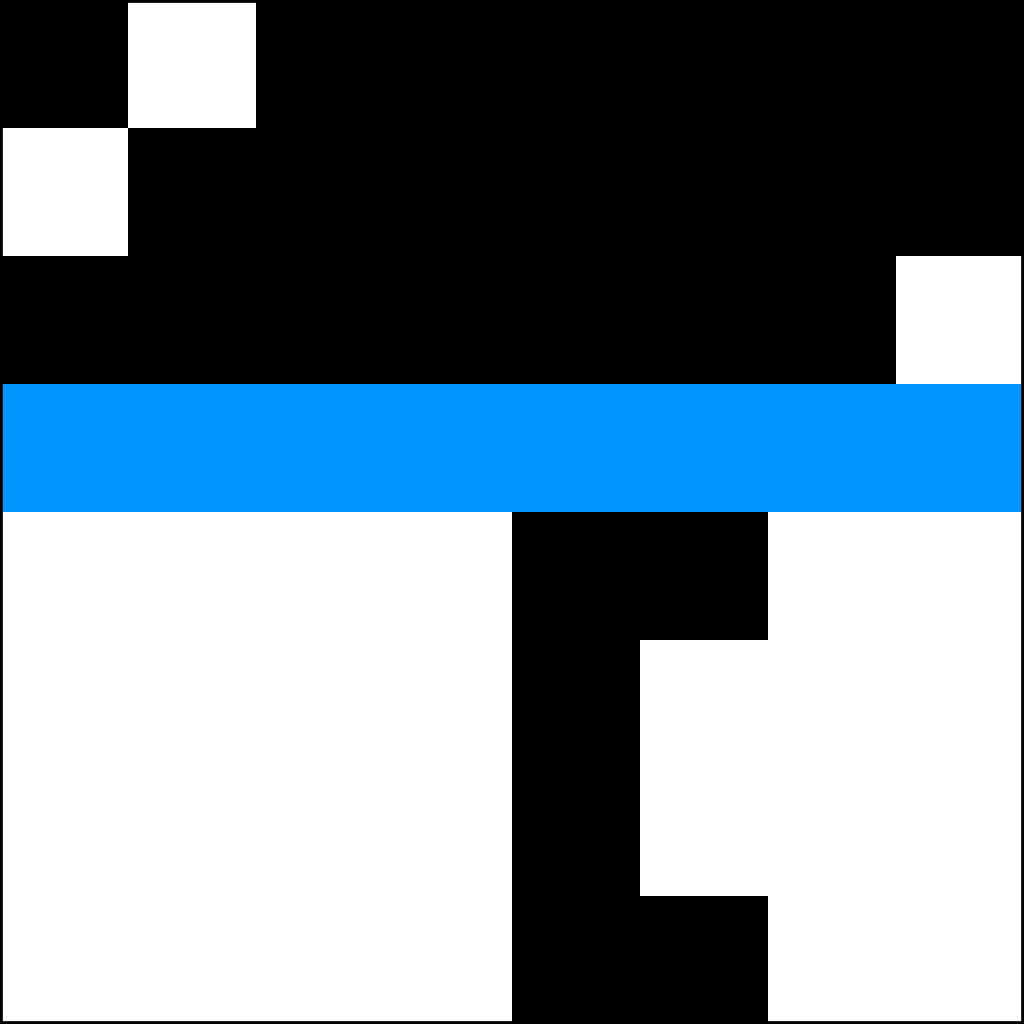
\includegraphics[width=3.1cm]{crossing-ex_perc2step3}
	\hspace{0.1cm}
	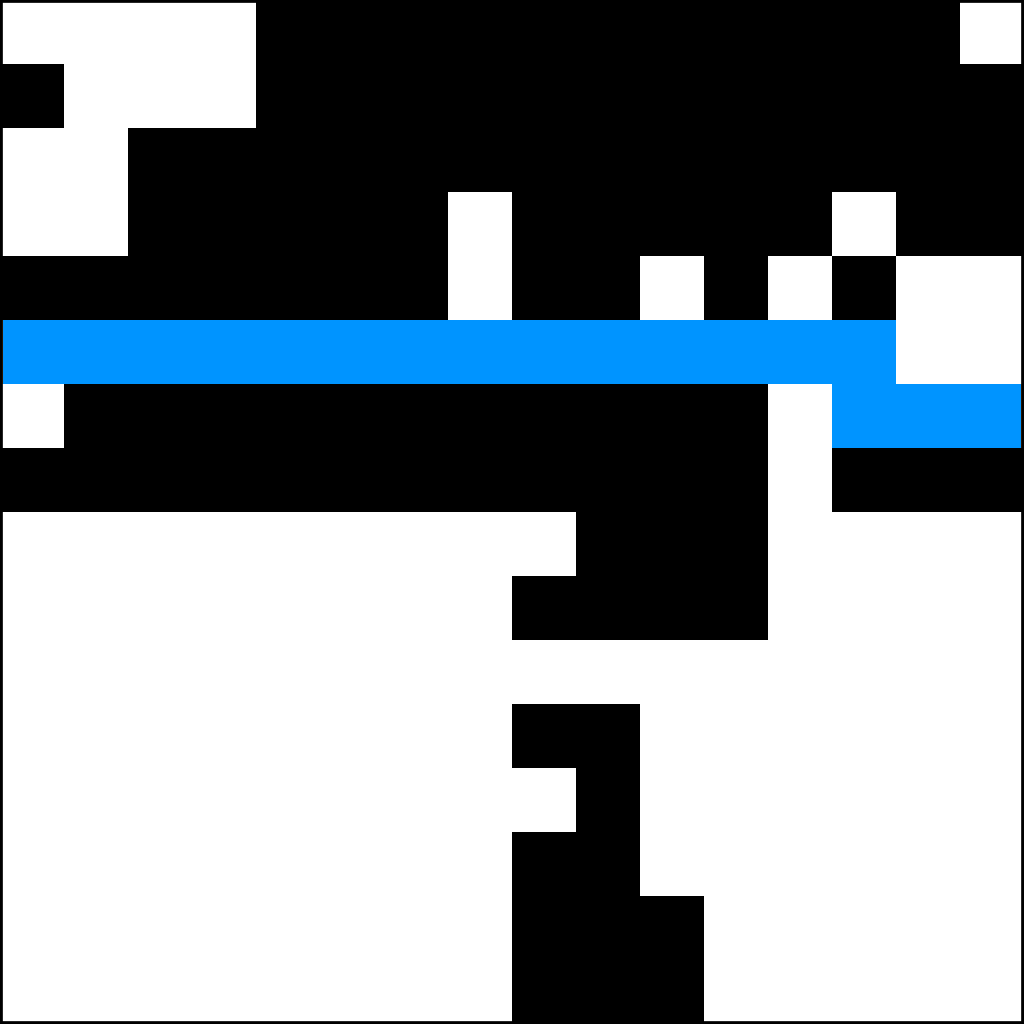
\includegraphics[width=3.1cm]{crossing-ex_perc2step4}
	\hspace{0.1cm}
	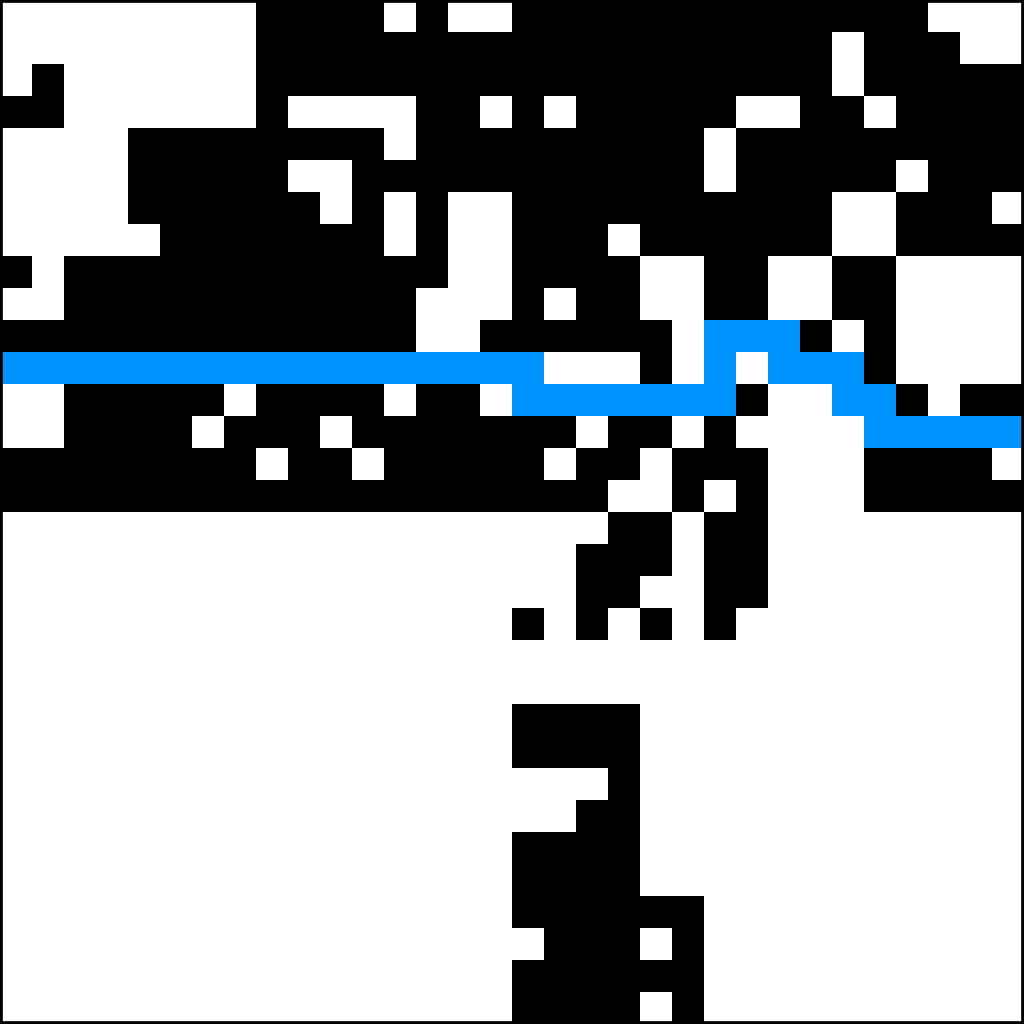
\includegraphics[width=3.1cm]{crossing-ex_perc2step5}
	\hspace{0.1cm}
	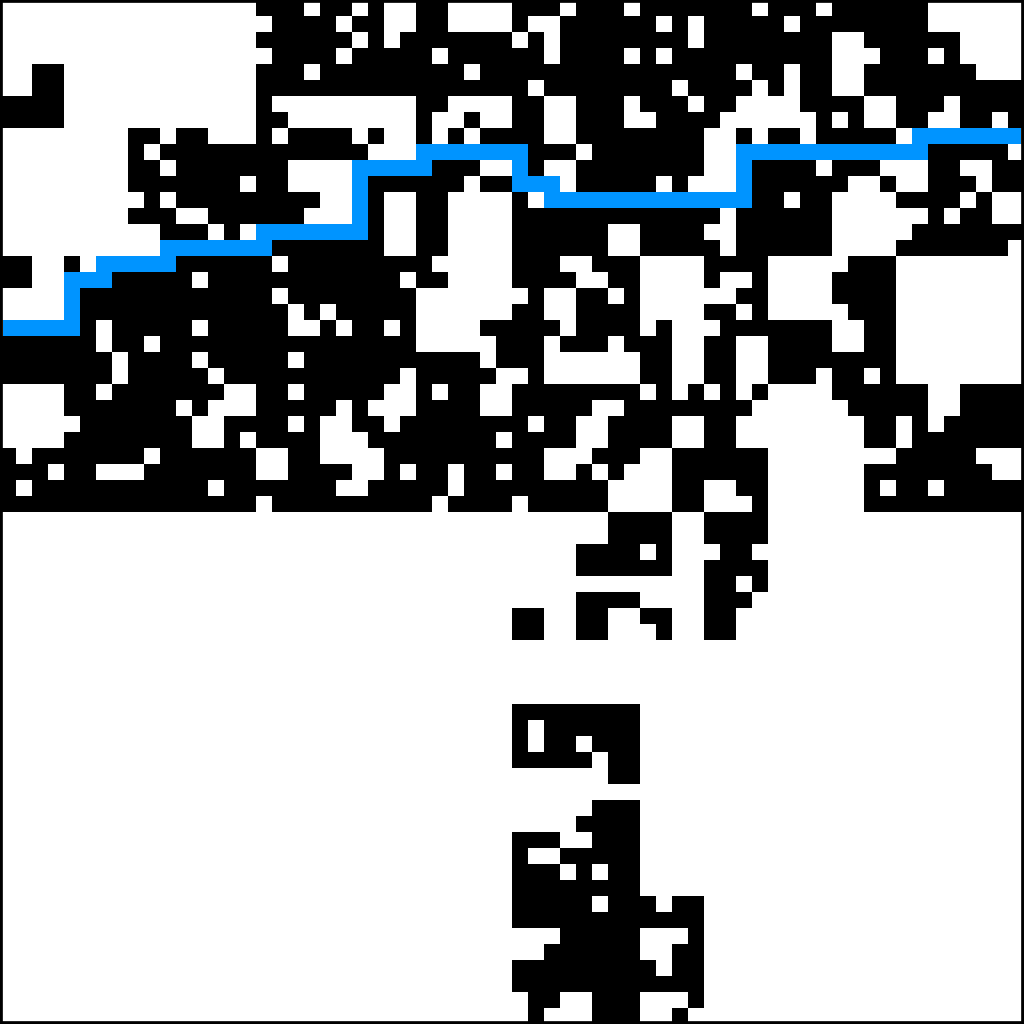
\includegraphics[width=3.1cm]{crossing-ex_perc2step6}
	\centering
	\caption{Crossings for a percolation with side $n=2$, at depths $k=2,3,4,5,6$.}
	\label{fig:crossingExPerc2}
\end{figure}
\begin{figure}[!h]
	
\includegraphics[width=4cm]{crossing-ex_perc3step1}
	\hspace{0.1cm}
	
\includegraphics[width=4cm]{crossing-ex_perc3step2}
	\hspace{0.1cm}
	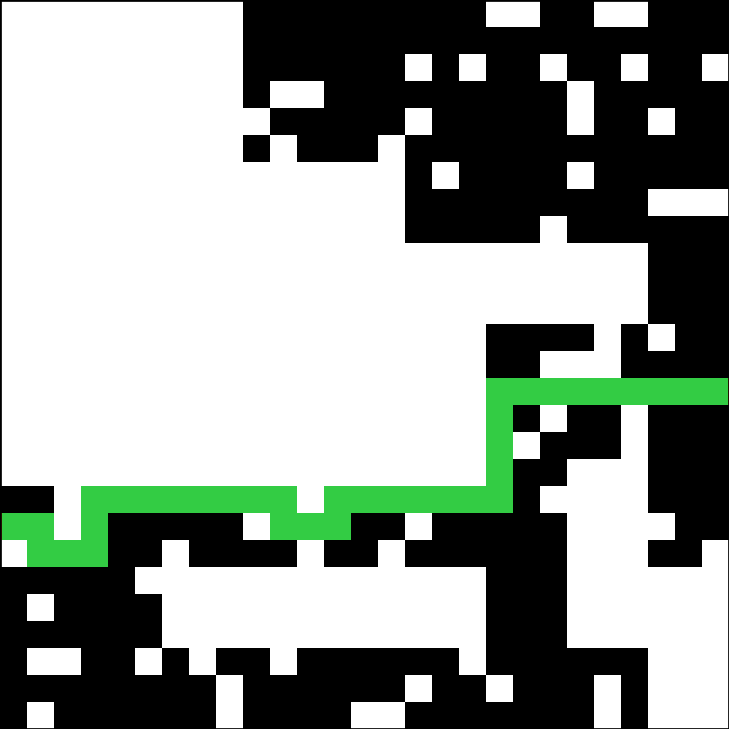
\includegraphics[width=4cm]{crossing-ex_perc3step3}
	\hspace{0.1cm}
	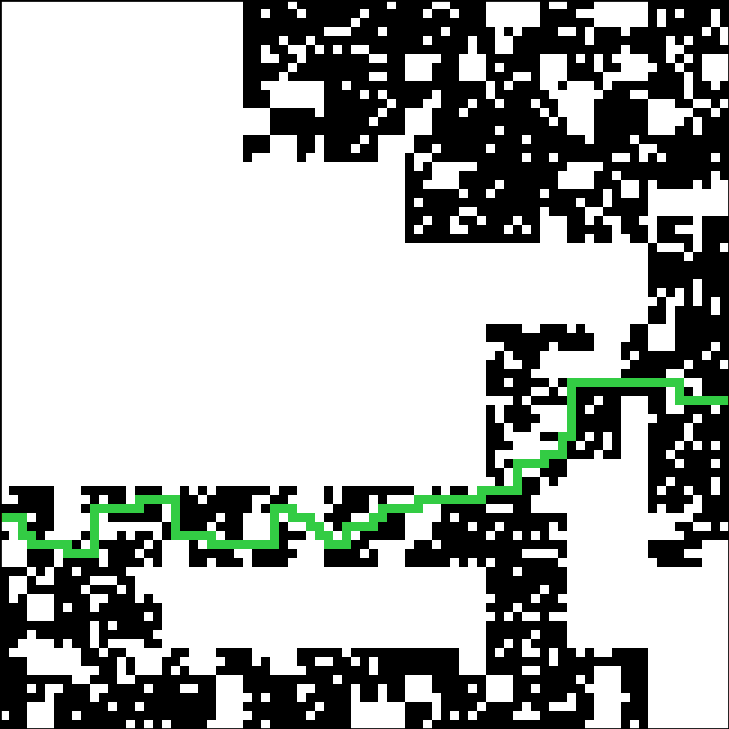
\includegraphics[width=4cm]{crossing-ex_perc3step4}
	\centering
	\caption{Crossings for a percolation with side $n=3$, at depths $k=1,2,3,4$.}
	\label{fig:crossingExPerc3}
\end{figure}
\begin{figure}[!h]
	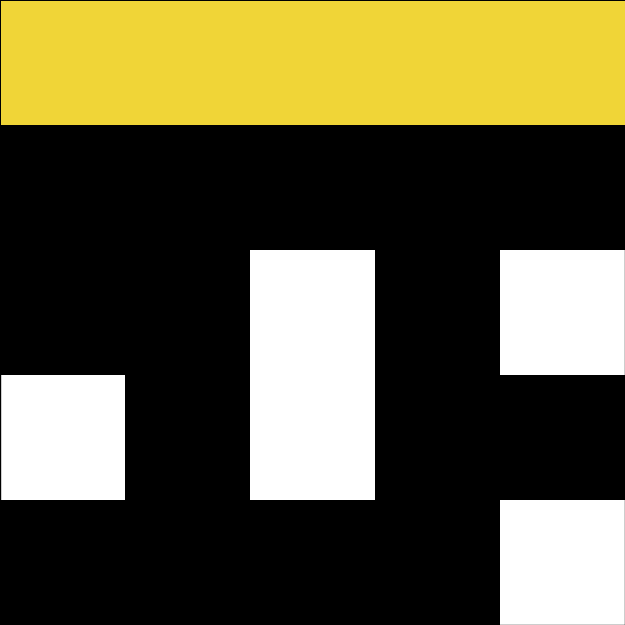
\includegraphics[width=4.9cm]{crossing-ex_perc5step1}
	\hspace{0.9cm}
	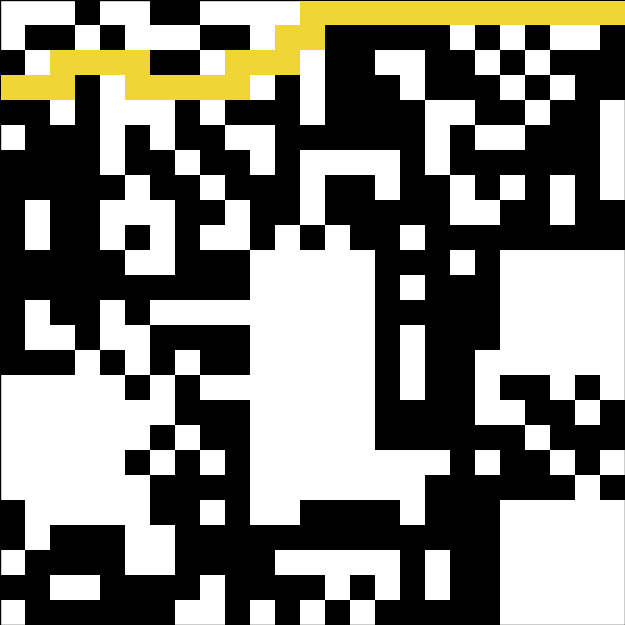
\includegraphics[width=4.9cm]{crossing-ex_perc5step2}
	\hspace{0.9cm}
	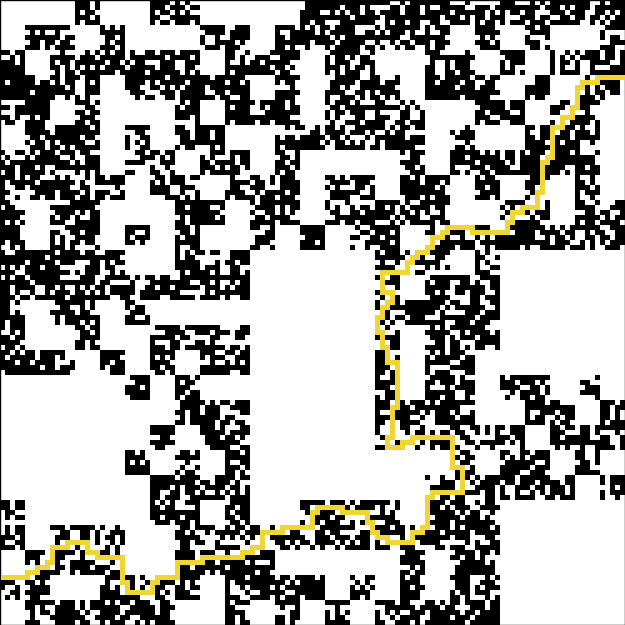
\includegraphics[width=4.9cm]{crossing-ex_perc5step3}
	\centering
	\caption{Crossings for a percolation with side $n=5$, at depths $k=1,2,3$.}
	\label{fig:crossingExPerc5}
\end{figure}

\paragraph{Algorithms}
\subparagraph{Percolations}
As (recursive) percolations are generated through a recursive process, it is logical (and elegant) to use a recursive function to generate them computationally.
We will represent a (finite) percolation $P \sim \text{Perc}^D(n,p,d)$ with a binary $D$-dimensional array of length $n^d$ in each dimensions.
Note that $D$ is a super-parameter.

This algorithm is given in pseudocode in algorithm \ref{algo:percolationGeneration}. Julia implementations
\footnote{2D percolation Julia implementation: \url{https://github.com/pauldubois98/PercolationFractalsStudy/blob/main/fractal\_percolation2D.jl}}
\footnote{3D percolation Julia implementation: \url{https://github.com/pauldubois98/PercolationFractalsStudy/blob/main/fractal\_percolation3D.jl}}
(used later in simulations for empirical estimations) can be found on the GitHub repository
\footnote{See \url{https://github.com/pauldubois98/PercolationFractalsStudy}.}.

\begin{algorithm}[!h]
	\caption{Percolation generation algorithm}\label{algo:percolationGeneration}
	\begin{algorithmic}[1]
		\State{\textit{Fills the $\left[ i_1,i_1+n^k\right] \times \cdots \times \left[ i_D,i_D+n^k\right]$ sub-array of $P$.}}
		\Procedure{percolationFill$^D$}{$P, \ i_1,\dots,i_D, \ n, p, k$}
		\If{$k = 0$}
		\State $P[i_1,\dots,i_D] \gets \textbf{random}()\footnotemark < p$ \Comment{stop recursion}
		\Else
		\For{$0 \leq j_1,\dots,j_D < n$}
		\If{$\textbf{random}() < p$}
		\State $\textsc{percolationFill}(P, \ i_1+(j_1 n^k),\dots,i_D+(j_D n^k), \ n, p, k-1)$ \Comment{recursion}
		\Else
		\State $P[i_1:i_1+n^k,\dots,i_D:i_D+n^k] \gets \textbf{zeros$^D$}(n^k,\dots,n^k)$ \Comment{void cells}
		\EndIf
		\EndFor
		\EndIf
		\EndProcedure
		\State{\textit{Generates a percolation $P \sim \text{Perc}^D(n,p,d)$.}}
		\Procedure{percolation$^D$}{$n, p, d$}
		\State $P \gets \textbf{init$^D$}(n^d,\dots,n^d)$
		\State $\textsc{percolationFill}(P, \ i_1,\dots,i_D, \ n, p, d)$ \Comment{fill $P$ recursively}
		\State \textbf{return} $P$
		\EndProcedure
	\end{algorithmic}
\end{algorithm}
\addtocounter{footnote}{-1}
\stepcounter{footnote}\footnotetext{$\textbf{random}()$ generates a random number $x \sim \mathcal{U}(0,1)$\footnotemark.}
\addtocounter{footnote}{-1}
\stepcounter{footnote}\footnotetext{Writing $x \sim \mathcal{U}(a,b)$ for $x$ a random variable with uniform distribution on $\left[ a,b \right]$.}

\subparagraph{Crossings}\label{crossingAlgorithm}
Given a percolation, it is not clear how to proceed on the task of determining if a crossing exists.

Our approach of the problem is rather unusual.

We simulate a "fire" propagating from one side of the cuboid, and check if it reaches the other side.\footnote{This is inspired by simulations of forest fires from the game "The Pyromaniac Game"\cite{pyromaniacGame}.}
If it does, then a crossing exists, otherwise, no crossing exists.
The rules of propagation for the fire (materialized by active cells\footnote{We call a "cell" one of the $D$ dimensional cuboids of side $\nicefrac{1}{n^d}$}) are as follows:
\begin{enumerate}
	\item If a cell is active at time $t$, then the non-empty adjacent cells become active at time $t+1$.
	\item If a cell is active at time $t$, it deactivates and can no longer be active on times $\tilde{t}>t$.
\end{enumerate}
At the beginning ($t=0$), we set all the non-empty cells from one side of the unit cuboid as active cells.
As soon as a cell from the opposite side of the unit cuboid is active, a path has been found (the time $t$ even gives the length of the crossing), and this is the shortest crossing.
If at some time $t$, no cell is active and no crossing was found before (i.e. the blaze turns off before reaching the other side), then no crossing exist.

Note that this technique tells us if there is a crossing, and what is the minimal length. However, it does not give the crossing path explicitly.
To find it, one needs to save the set of active cells at each time, and propagate backwards.

This algorithm \ref{algo:crossingFinding} is a pseudocode implementation of this process.
Julia implementations
\footnote{2D crossing Julia implementation: \url{https://github.com/pauldubois98/PercolationFractalsStudy/blob/main/crossings2D.jl}}
\footnote{3D crossing Julia implementation: \url{https://github.com/pauldubois98/PercolationFractalsStudy/blob/main/crossings3D.jl}}
(used for empirical probability approximation) can be found again on the GitHub repository
\footnote{See \url{https://github.com/pauldubois98/PercolationFractalsStudy}.}.

Visualisation of this algorithm:
\begin{itemize}
	\item In 2D: \url{https://pauldubois98.github.io/PercolationFractalsAlgorithmsDemo/2Dcrossing/index.html}
	\item In 3D: \url{https://pauldubois98.github.io/PercolationFractalsAlgorithmsDemo/3Dcrossing/index.html}
\end{itemize}

\begin{algorithm}[!h]
	\caption{Crossing finding algorithm}\label{algo:crossingFinding}
	\begin{algorithmic}[1]
		\State{\textit{Perform one step propagation on $A$, with respect to $P$}}
		\Procedure{neighbors$^D$}{$A,\, P, \ n,d$}
		\State $B \gets \textbf{zeros$^D$}(n^d,\dots,n^d)$ \Comment{newly active cells}
		\For{$1 \leq i_1,\dots,i_D < n^d$}
		\If{$A[i_1,\dots,i_D]=2$}
		\State $B[i_1,\dots,i_D] = 2$ \Comment{remain inactive}
		\EndIf
		\If{$A[i_1,\dots,i_D]=1$}
		\State $B[i_1,\dots,i_D] = 2$ \Comment{deactivate cell}
		\For{$1 \leq j \leq D$}
		\If{$P[i_1,\dots,i_j-1,\dots,i_D]$ and $A[i_1,\dots,i_j-1,\dots,i_D] = 0$}
		\State $B[i_1,\dots,i_j-1,\dots,i_D] \gets 1$ \Comment{activate cell}
		\EndIf
		\If{$P[i_1,\dots,i_j+1,\dots,i_D]$ and $A[i_1,\dots,i_j+1,\dots,i_D] = 0$}
		\State $B[i_1,\dots,i_j+1,\dots,i_D] \gets 1$ \Comment{activate cell}
		\EndIf
		\EndFor
		\EndIf
		\EndFor
		\State \textbf{return} $B$
		\EndProcedure
		\State{\textit{Returns the length of the shortest crossing on percolation $P \sim \text{Perc}^D(n,p,d)$; returns $0$ if none exist.}}
		\Procedure{crossing$^D$}{$P,\ n,d$}
		\State $A \gets \textbf{zeros$^D$}(n^d,\dots,n^d)$ \Comment{active cells}
		\State $A[0,:,\dots,:] \gets P[0,:,\dots,:]$ \Comment{initialize active cells}
		\State $t \gets 0$
		\While{\textbf{any}($A=1$) and \textbf{any}($A[n^d,:,\dots,:]=1$)}
		\State $A \gets \textsc{neighbors}(P,A)$ \Comment{propagate one step}
		\State $t \gets t+1$
		\EndWhile
		\If{\textbf{any}$(A[n^d,:,\dots,:])$}
		\State \textbf{return} $t$
		\Else
		\State \textbf{return} $0$
		\EndIf
		\EndProcedure
	\end{algorithmic}
\end{algorithm}

By restricting the possible steps (not allowing activation to propagate backwards), this algorithm may be adapted to find semi-straight crossings (the above would give non-straight crossings).
It can also be used for straight crossings, but in this case, it is faster to sum the percolation array on the first dimension: a straight crossing exists if one of the sums gives $n^d$.

%implementation choices